\documentclass[11pt]{article}

\usepackage{amsmath,amssymb}
\usepackage{booktabs}
\usepackage{graphicx}
\usepackage{geometry}
\usepackage{siunitx}
\geometry{margin=1.1in}

\title{Bayesian Estimation of \texttt{mmt8bOccBin3\_covid\_bT\_baa}:\\
Methodology, Convergence, and Determinacy/E-Stability Results}
\author{}
\date{\today}

\begin{document}
\maketitle

\begin{abstract}
This note documents the Bayesian estimation of an extended version of the
shopping-time/banking-sector model with monetary and fiscal policy
interactions, adding (i) an endogenous debt-to-GDP ratio observable built
from FRED federal debt held by the public and nominal GDP, (ii) a Baa
corporate bond yield in place of the bank-prime rate for the loan-rate
observable, (iii) a genuine OccBin piecewise-linear zero-lower-bound
(ZLB) likelihood in place of a linear-Kalman-filter approximation, and
(iv) a single independent, identically distributed (iid) shock to the
labor-leisure margin standing in for the COVID-19 labor-supply collapse.
This round additionally recalibrates two structural parameters --
the steady-state tax target $\bar\tau$ (from 0.20 to 0.14, implying a
6\%-of-GDP steady-state deficit, more realistic than the previous
$\approx$0\% balanced-budget target) and the shopping-time curvature
$\chi$ (from 1.0 to 0.5, chosen after comparative-statics checks showed
it substantially lowers steady-state inflation via higher money demand)
-- both of which shift the model's steady state and require re-running
mode-finding and estimation from scratch. We report the two-stage
mode-finding and jump-scale tuning -- including a switch from a diagonal
(\texttt{prior\_variance}) to a Hessian-based MCMC jumping covariance,
adopted in an earlier round to resolve a chain-disagreement problem that
produced bimodal-looking pooled posterior densities, and a further
switch to a jumping covariance built directly from a preliminary round's
own pooled posterior draws once the Hessian-based approach itself began
showing renewed (if milder) chain disagreement under the recalibrated
model -- used to obtain a well-mixing Markov chain Monte Carlo (MCMC)
sample under OccBin's nonsmooth likelihood, the resulting posterior
distribution and Geweke
(1992) convergence diagnostics, a determinacy and
expectational-stability (E-stability) map for the non-ZLB (RELAX) regime
evaluated at the posterior means, and a table of annualized steady-state
rates implied by those estimates.

\textbf{This revision reports a further re-estimation round} on top of
the above, prompted by two changes: (i) a corrected household
budget-constraint identity for reserves $n_t$, which previously used a
fixed steady-state placeholder for the debt terms rather than the
genuine (lagged and current) debt state, and (ii) substantially less
informative priors on the Taylor-rule policy-response coefficients
$b_\pi$ and $b_y$ (Gamma(1.00, 1.00) and Gamma(1.00, 0.70), replacing a
tight Normal(2.10, 0.15) and Gamma(0.28, 0.10) respectively) together
with a lower prior mean for the fiscal-feedback parameter $\varphi_b$
(0.05, from 0.10), so that the posterior on the inflation-response
coefficient in particular reflects what the data support rather than a
tight prior. All posterior, convergence, determinacy, and steady-state
results reported below are from this latest round; the tuning history
of the earlier (tight-prior) round is retained for context.
\end{abstract}

\section{Model Extensions}

The estimated model, \texttt{mmt8bOccBin3\_covid\_bT\_baa.mod}, extends
the baseline quarterly \texttt{mmt8bOccBin3} specification along four
dimensions.

\paragraph{Debt-to-GDP observable.} An endogenous debt-to-GDP ratio is
added as
\[
bT_t = \frac{b_t}{1+g},
\]
where $b_t$ is the model's real net-debt-to-output ratio and $g$ is
steady-state government spending as a share of output (so $1+g$
approximates steady-state GDP in the model's units). The corresponding
observable is
\[
bT^{obs}_t = \log(bT_t) - \log\!\big(\overline{bT}\big) + \varepsilon^{bT}_{me,t},
\]
built from FRED series \texttt{FYGFDPUN} (federal debt \emph{held by the
public}, not gross/total public debt) divided by \texttt{GDP} (nominal
GDP), log-demeaned over the sample. An earlier version of this
observable used \texttt{GFDEBTN} (total public debt) and demeaned in
levels rather than logs, inconsistent with the measurement equation
above; both issues are fixed in the current data build (see
Section~\ref{sec:data}).

\paragraph{Baa-based loan rate.} The loan-rate observable $r^{obs}_t$ is
constructed from Moody's Seasoned Baa Corporate Bond Yield (FRED series
\texttt{BAA}) rather than the bank prime rate (\texttt{MPRIME}) used in
earlier versions of this model. The Baa series carries genuine
credit-spread variation (widening in recessions, narrowing in
recoveries) instead of being mechanically pinned to the federal funds
rate plus a fixed spread, and its 2009--2025 sample average sits closer
to the model's steady-state loan rate.

\paragraph{Genuine OccBin ZLB likelihood.} The interest-rate rule on
reserves is subject to a zero lower bound,
\[
r^n_t = \max\!\Big[1,\; (r^{\ell}_t)^{a_i}\Big(\frac{\pi_t}{\pi}\Big)^{b_\pi}
\Big(\frac{y_t}{y}\Big)^{b_y} e^{z^r_t}\Big],
\]
implemented via Dynare's \texttt{occbin\_constraints} block. Earlier
versions of this file carried the \texttt{occbin\_constraints}
specification syntactically but disabled OccBin's piecewise-linear
Kalman filter and smoother at estimation time
(\texttt{options\_.occbin.likelihood.status = false}), falling back to a
standard linear filter that ignores the bound. This estimation instead
sets \texttt{options\_.occbin.likelihood.status = true} together with
\texttt{options\_.occbin.smoother.periodic\_solution = true} and
\texttt{options\_.occbin.regularisation = 1e{-}3}, so the likelihood
genuinely enforces the ZLB across both binding episodes in the sample
(2009Q1--2015Q4 and 2020Q1--2021Q4).

\paragraph{COVID labor-supply shock.} Rather than reproduce the
multi-shock, regime-switching COVID mechanism of Cardani, Pfeiffer,
Ratto, and Vogel (2023), the model adds a single iid shock $\varepsilon^L_t$
to the household labor-leisure first-order condition,
\[
\frac{c_t}{z}h_t^{\psi} + \chi\, hs_t = \frac{1}{\eta}\exp(\varepsilon^L_t),
\]
with $\varepsilon^L_t \sim N(0,\sigma_L^2)$ and $\sigma_L$ estimated. A
negative realization of $\varepsilon^L_t$ shrinks the right-hand side,
forcing lower labor supply for given consumption and wages -- a negative
labor-supply shock. A deterministic one-period dummy
(\texttt{varexo\_det}) was considered first, matching a specific
calendar quarter, but Dynare 7.1's estimation routine
(\texttt{dynare\_estimation\_init.m}) does not read \texttt{varexo\_det}
variables from the estimation data file, so such a dummy would be
silently ignored by the Kalman filter. The iid \texttt{varexo} shock
avoids this and lets the smoother (when it converges) attribute
whatever realization the data require to the appropriate quarter without
a hardcoded date.

\paragraph{Recalibration: $\bar\tau$ and $\chi$.} Two calibrated (not
estimated) structural parameters were revised this round.
\emph{$\bar\tau$}: the steady-state tax target, entering the tax rule
\[
\tau_t = \tau_{t-1}^{\rho_\tau}\,\bar\tau^{1-\rho_\tau}
\Big(\frac{b_{t-1}}{(1-\omega)b_0}\Big)^{\varphi_b} e^{\varepsilon^\tau_t},
\]
was lowered from 0.20 to 0.14. Because government spending is fixed at
$g=0.2$, the steady state satisfies $\tau_{ss}=\bar\tau$ exactly and
$b_{ss}=b_0$ exactly (verified numerically), so the steady-state deficit
$g-\bar\tau$ moved from $\approx$0\% to 6\% of GDP -- a more realistic
target for the 2009--2025 sample away from the ZLB than a balanced
budget. Comparative statics at the previous round's posterior means
showed this relationship is steep: at $\bar\tau=0.15$, steady-state
annual inflation was 8.66\%; at $\bar\tau=0.12$, 15.85\%; at
$\bar\tau=0.05$ the steady-state solver failed to converge at all,
consistent with the model approaching the peak of its seigniorage
(Laffer-type) curve. \emph{$\chi$}: the shopping-time curvature
parameter in $hs_t=(1/\chi)(v_{a,t}c_t/d_t)^\chi$, was lowered from 1.0
to 0.5. A comparative-statics sweep ($\chi\in[0.3,2.0]$, other
parameters at the previous round's posterior means) showed a smooth,
monotonic relationship between $\chi$ and steady-state inflation --
lower $\chi$ raises real money demand substantially (roughly 8-fold
from $\chi=2.0$ to $\chi=0.3$ in that sweep), which lowers the inflation
tax needed to finance a given deficit. Both parameters remain calibrated
rather than added to \texttt{estimated\_params}.

\paragraph{Reserve equation fix: genuine debt-state coupling.} The
equation linking reserves $n_t$ to currency and debt (the model's analog
of the household budget-constraint identity $n_t = m_{t-1}/\Pi_t +
b_{t-1}/\Pi_t - b_t/r_t$) previously read
\[
n_t = \frac{m_{t-1}}{\pi_t} + b_0(1-\omega)\Big(\frac{1}{\pi_t}-\frac{1}{r^\ell_t}\Big),
\]
using the fixed steady-state debt target $b_0(1-\omega)$ in place of the
actual (lagged and current) debt state -- meaning $n_t$ never responded
to fluctuations in outstanding debt at all. This is corrected to
\[
n_t = \frac{m_{t-1}}{\pi_t} + \frac{b_{t-1}}{\pi_t} - \frac{b_t}{r^\ell_t},
\]
the model's direct analog of the theoretical identity. This is safe for
Blanchard-Kahn purposes because $b_t$'s own law of motion (the
debt-issuance equation, which fixes the $r^\ell_t/\pi_t$ ratio at its
steady-state value $r^{\ell,ss}/\pi^{ss}$ for exactly this reason) never
depends on any forward-looking variable, so it remains a purely
backward/exogenous recursion regardless of where else it appears
contemporaneously. Verified directly: steady-state values and the
Blanchard-Kahn eigenvalue count (4 forward-looking variables, order and
rank conditions satisfied) are unchanged before and after the fix.

\paragraph{Less informative Taylor-rule priors.} The priors on the
inflation- and output-response coefficients, $b_\pi$ and $b_y$, were
loosened substantially -- from Normal(2.10, 0.15) and Gamma(0.28, 0.10)
to Gamma(1.00, 1.00) and Gamma(1.00, 0.70) respectively -- so that the
posterior is not mechanically dominated by a tight prior centered near
the previous round's own answer. A first attempt used Gamma(1.00, 1.00)
(shape 1, i.e.\ Exponential(1)) for both; $b_\pi$'s posterior moved away
from the prior's mode at zero without difficulty, but $b_y$'s mode
landed at exactly 0.0000 with a non-positive-definite Hessian there --
a corner solution the shape-1 prior itself pre-loads, since an
Exponential density is maximized at zero. $b_y$'s prior was reshaped to
Gamma(1.00, 0.70) (shape $\approx$2.04, an interior mode near 0.51, no
boundary pre-loading) while keeping the same diffuse mean, which
resolved this. The fiscal-feedback parameter $\varphi_b$'s prior mean
was also lowered, from 0.10 to 0.05, keeping its prior standard
deviation (0.05) unchanged.

\subsection{Summary of stochastic elements}
\label{sec:shocksummary}

Table~\ref{tab:shocks} consolidates every stochastic element in the
model -- the eight structural shocks discussed above and the seven
measurement-error shocks attached to the observable equations -- in one
place, since the discussion above introduces each one individually at
the point it enters the model rather than as a single reference list.

\begin{table}[h]
\centering
\small
\begin{tabular}{@{}llll@{}}
\toprule
Symbol & Affects & Law of motion & Persistence \\
\midrule
\multicolumn{4}{@{}l}{\textit{Structural shocks}} \\
$\varepsilon_{a,t}$   & Preference wedge $a_t$ (eq. \ref{U})        & $a_t=a_{t-1}^{\rho_a}\exp(\varepsilon_{a,t})$ & $\rho_a=0.95$ \\
$\varepsilon_{z,t}$   & Productivity $z_t$ (eq.~prod)         & $z_t=z_{t-1}^{\rho_z}z^{1-\rho_z}\exp(\varepsilon_{z,t})$ & $\rho_z$ estimated \\
$\varepsilon_{va,t}$  & Shopping-time pref.\ $v_{a,t}$ (eq.~hs) & $v_{a,t}=v_{a,t-1}^{\rho_{va}}v_a^{1-\rho_{va}}\exp(\varepsilon_{va,t})$ & $\rho_{va}=0$ \\
$\varepsilon_{xa,t}$  & Deposit technology $x_{a,t}$ (eq.~d)   & $x_{a,t}=x_{a,t-1}^{\rho_{xa}}x_a^{1-\rho_{xa}}\exp(\varepsilon_{xa,t})$ & $\rho_{xa}=0.95$ \\
$\varepsilon_{g,t}$   & Govt.\ spending $g_t$ (resource constr.) & $g_t=\rho_g g_{t-1}+(1-\rho_g)g+\varepsilon_{g,t}$ & $\rho_g=0$ \\
$\varepsilon^r_t$     & MP shock $z^r_t$ (Taylor rule)         & $z^r_t=b_r z^r_{t-1}+\varepsilon^r_t$ & $b_r$ estimated \\
$\varepsilon^\tau_t$  & Tax rule (eq.~tau)                     & iid & -- \\
$\varepsilon^L_t$     & Labor-leisure FOC (COVID stand-in)     & iid & -- \\
\midrule
\multicolumn{4}{@{}l}{\textit{Measurement-error shocks (one per observable, all iid)}} \\
$\varepsilon^{me}_{y,t}$    & $y^{obs}_t$ (output)              & -- & -- \\
$\varepsilon^{me}_{d,t}$    & $d^{obs}_t$ (deposits)            & -- & -- \\
$\varepsilon^{me}_{\pi,t}$  & $\pi^{obs}_t$ (inflation)         & -- & -- \\
$\varepsilon^{me}_{r,t}$    & $r^{obs}_t$ (loan rate)           & -- & -- \\
$\varepsilon^{me}_{r^n,t}$  & $r^{n,obs}_t$ (policy rate)       & -- & -- \\
$\varepsilon^{me}_{\tau,t}$ & $\tau^{obs}_t$ (tax rate)         & -- & -- \\
$\varepsilon^{me}_{bT,t}$   & $bT^{obs}_t$ (debt/GDP)           & -- & -- \\
\bottomrule
\end{tabular}
\caption{All fifteen stochastic elements of the estimated model.
``Persistence'' reports whether the process's own AR(1) coefficient is
fixed by calibration or freely estimated; iid processes (measurement
errors and three of the structural shocks) have no persistence
parameter. Standard deviations, priors, and posterior estimates for all
fifteen are in Table~\ref{tab:posteriors}.}
\label{tab:shocks}
\end{table}

Eight of the fifteen are structural, entering the model's own equations
and so shaping the dynamics of $y_t,\pi_t,r^\ell_t,\ldots$ directly;
seven are measurement error, entering only the observation equations
that link model variables to the FRED data series (Table~\ref{tab:data}
below) and therefore affecting the likelihood but not the model's own
propagation mechanism. Of the eight structural shocks, persistence
splits four ways: $\varepsilon^\tau_t$ and $\varepsilon^L_t$ have no
persistence parameter at all (direct iid entry); $v_{a,t}$ and $g_t$
are written with an AR(1) law of motion but have that persistence fixed
at exactly zero (functionally iid); $a_t$ and $x_{a,t}$ have persistence
fixed at a nonzero value, $\rho_a=\rho_{xa}=0.95$ (freeing them
previously drove $\rho_a$ to a near-unit-root value and produced a
non-positive-definite Hessian, Section~2.2); and $z_t$ and $z^r_t$ have
their persistence ($\rho_z$, $b_r$) freely estimated.

\section{Estimation Methodology}

\subsection{Data}
\label{sec:data}
The model is estimated on seven quarterly U.S. observables spanning
2009Q1--2025Q4 (68 observations), all sourced from the Federal Reserve
Bank of St.\ Louis FRED database. Series reported at a higher frequency
(monthly or weekly) are averaged to quarterly. Every series is demeaned
by its own full-sample mean prior to estimation (in logs, consistently
with every measurement equation), matching the model's measurement
equations, which express each observable as a log-deviation from steady
state plus measurement error. Table~\ref{tab:data} lists the
construction of each series; currency in circulation, used as an eighth
observable in earlier versions of this model, is excluded here.

\begin{table}[h]
\centering
\small
\begin{tabular}{@{}lll@{}}
\toprule
Observable & FRED series & Transformation \\
\midrule
$y^{obs}$ (output) & \texttt{GDPC1} / \texttt{OPHNFB} &
  $\log(\text{GDPC1}/\text{OPHNFB})$, demeaned \\
$d^{obs}$ (deposits) & \texttt{DPSACBW027SBOG} / \texttt{OPHNFB} &
  $\log(\text{Deposits}/\text{OPHNFB})$, demeaned \\
$\pi^{obs}$ (inflation) & \texttt{GDPDEF} &
  $\log(\text{GDPDEF}_t/\text{GDPDEF}_{t-1})$, demeaned \\
$r^{obs}$ (loan rate) & \texttt{BAA} &
  $\log(1+\text{BAA}_q/400)$, demeaned \\
$r^{n,obs}$ (policy rate) & \texttt{FEDFUNDS} &
  $\log\!\big((1+\text{FEDFUNDS}/100)^{0.25}\big)$, demeaned \\
$\tau^{obs}$ (tax rate) & \texttt{FGRECPT} / \texttt{GDP} &
  $\log(\text{Tax receipts}/\text{Nominal GDP})$, demeaned \\
$bT^{obs}$ (debt/GDP) & \texttt{FYGFDPUN} / \texttt{GDP} &
  $\log\big((\text{FYGFDPUN}/1000)/\text{GDP}\big)$, demeaned \\
\bottomrule
\end{tabular}
\caption{Observable construction. \texttt{OPHNFB} is nonfarm business
sector output per hour (labor productivity), used to detrend output and
deposits. \texttt{BAA} (Moody's Seasoned Baa Corporate Bond Yield,
monthly) replaces the bank prime rate (\texttt{MPRIME}) used in earlier
versions of this model. \texttt{FYGFDPUN} (Federal Debt Held by the
Public, quarterly, millions of dollars) replaces \texttt{GFDEBTN}
(gross/total public debt); it is divided by 1000 before forming the
ratio because \texttt{FYGFDPUN} is reported in millions of dollars while
\texttt{GDP} is reported in billions. $q$ subscripts denote quarterly
averages of monthly series.}
\label{tab:data}
\end{table}

\emph{Data-provenance notes.} Two issues were found and fixed while
rebuilding this observable. First, \texttt{NGDPDQ} -- referenced as the
GDP denominator in an earlier data-fetch script's header comments and in
this model file's own prior header -- is not a valid FRED series
(\texttt{fredgraph.csv?id=NGDPDQ} returns an HTML error page, not data);
the debt-to-GDP data actually used in earlier estimation rounds came
from a separately pre-downloaded ratio file, not from that script. The
nominal-GDP denominator is now \texttt{GDP}, the same series already
used correctly elsewhere in this pipeline for $\tau^{obs}$. Second, the
measurement equation for $bT^{obs}_t$ is a log-deviation, but the
data-construction scripts used in earlier rounds demeaned the raw ratio
in \emph{levels} instead; the current build demeans in logs, matching
the model.

\subsection{Two-stage mode-finding}
OccBin's piecewise-linear likelihood is nonsmooth at ZLB regime
switches, and gradient-based optimizers such as \texttt{csminwel} tend
to fail on it directly. Estimation therefore proceeds in two stages,
repeated whenever the observation data \emph{or} the calibration
changes (mode-finding depends on the likelihood, which depends on both,
even when the model equations themselves are unchanged):

\begin{enumerate}
\item \textbf{Stage 1 (linear Kalman filter).} With
\texttt{options\_.occbin.likelihood.status = false}, the posterior mode
is located with \texttt{mode\_compute=4} (\texttt{csminwel}). An initial
attempt that additionally freed the productivity persistence parameters
$\rho_a,\rho_{xa}$ (previously fixed at 0.95 in the baseline model)
converged to $\rho_a \approx 0.9992$ -- effectively a unit root -- and
produced a non-positive-definite Hessian at the mode; $\rho_a=\rho_{xa}=0.95$
have been fixed (not estimated) ever since. Under the current
calibration ($\bar\tau=0.14$, $\chi=0.5$), Stage 1 mode-finding again
produced a positive-definite Hessian with no singularity warnings,
acceptance ratios 0.223/0.230 on a short diagnostic run (informational
only, since this stage still uses the linear, non-OccBin,
approximation).
\item \textbf{Stage 2 (true OccBin likelihood).} With
\texttt{options\_.occbin.likelihood.status = true}, estimation is
restarted at \texttt{mode\_compute=0} using the Stage 1 mode as the
starting point. A mode file computed under a different parameter vector
\emph{or} different data/calibration causes Dynare to throw ``generated
using another specification of the model'' (in the parameter-vector
case) or simply to start MCMC from a stale, no-longer-optimal point (in
the data/calibration-change case, which Dynare's compatibility check
does not catch and must be tracked manually) -- Stage 1's mode, rebuilt
under the identical parameter vector and current data/calibration,
avoids both.
\end{enumerate}

\subsection{MCMC jumping covariance and jump-scale tuning}
\label{sec:jumpcov}
An initial production run under the previous calibration
($\bar\tau=0.20$, $\chi=1.0$, \texttt{mh\_jscale=0.02},
\texttt{mcmc\_jumping\_covariance=prior\_variance}) passed the
0.05-acceptance-ratio floor (0.271/0.242) but produced posterior
densities for three of the four policy parameters ($b_\pi$, $b_y$,
$\varphi_b$) that visibly appeared bimodal when the two chains' draws
were pooled. Checking the two chains separately showed this was chain
disagreement, not genuine multimodality (chain means 1.86 and 1.67
pooled standard deviations apart for $b_\pi$, $b_y$ respectively, each
chain individually unimodal and tight) -- consistent with
\texttt{prior\_variance}'s diagonal proposal covariance ignoring the
$b_\pi$/$b_y$ correlation inherent to Taylor-rule estimation.

Switching \texttt{mcmc\_jumping\_covariance} to \texttt{hessian} (using
the Stage-1 mode's Hessian, which captures this correlation) fixed the
chain-disagreement problem in the subsequent round (under
$\bar\tau=0.20$, \texttt{FYGFDPUN}-based data), but required extensive
\texttt{mh\_jscale} re-tuning from scratch, including one attempt
(\texttt{mh\_jscale=1.0}) that produced 6{,}861 near-singular-matrix
warnings and took over an hour without finishing 3{,}000 draws, and
repeated cases where short (3{,}000-draw) diagnostics overstated what a
full 50{,}000-draw production run would sustain. Table~\ref{tab:jscale}
reports the full history across all rounds; for the current calibration
($\bar\tau=0.14$, $\chi=0.5$), the \texttt{mh\_jscale=0.10} setting that
had worked previously was tried directly as an informed first guess and
succeeded on the first production attempt (0.1775/0.1534), the first
round not requiring a kill-and-retune cycle.

\begin{table}[h]
\centering
\small
\begin{tabular}{@{}llccl@{}}
\toprule
Jumping covariance & \texttt{mh\_jscale} & Chain 1 & Chain 2 & Outcome \\
\midrule
\multicolumn{5}{@{}l}{\textit{$\bar\tau=0.20$, $\chi=1.0$; debt observable: GFDEBTN, level-demeaned}} \\
\texttt{prior\_variance} & 0.05 & 0.0433 & 0.0710 & Chain 1 below 0.05 -- killed \\
\texttt{prior\_variance} & 0.03 (diag., 3k) & 0.203 & 0.057 & Both above 0.05 -- promoted \\
\texttt{prior\_variance} & 0.03 (prod., 50k) & 0.157 & 0.0477 & Chain 2 below 0.05 -- killed \\
\texttt{prior\_variance} & 0.02 (diag., 3k) & 0.306 & 0.293 & Both healthy -- promoted \\
\texttt{prior\_variance} & 0.02 (prod., 50k) & 0.271 & 0.242 & Accepted; bimodal pooled densities \\
\midrule
\multicolumn{5}{@{}l}{\textit{$\bar\tau=0.20$, $\chi=1.0$; debt observable: FYGFDPUN/GDP, log-demeaned}} \\
\texttt{hessian} & 1.0 (diag., 3k) & 0.0073 & 0.0040 & Both far below 0.05; 6{,}861 singular warnings, $>$1hr -- killed \\
\texttt{hessian} & 0.2 (diag., 3k) & 0.100 & 0.104 & Both healthy on diagnostic -- promoted \\
\texttt{hessian} & 0.2 (prod., 50k) & 0.0449 & 0.0582 & Chain 1 below 0.05; took 15h03m -- killed \\
\texttt{hessian} & 0.12 (diag., 3k) & 0.122 & 0.129 & Both healthy -- extra margin sought \\
\texttt{hessian} & 0.10 (diag., 3k) & 0.236 & 0.265 & Both in textbook 0.2--0.4 range -- promoted \\
\texttt{hessian} & 0.10 (prod., 50k) & 0.214 & 0.195 & Accepted \\
\midrule
\multicolumn{5}{@{}l}{\textit{$\bar\tau=0.14$, $\chi=0.5$; debt observable: FYGFDPUN/GDP, log-demeaned}} \\
\texttt{hessian} & 0.10 (diag., 3k) & 0.405 & 0.259 & Both healthy, good margin -- promoted \\
\texttt{hessian} & 0.10 (prod., 50k) & 0.1775 & 0.1534 & Accepted, but Geweke uneven (\S\ref{sec:geweke}) \\
\texttt{posterior-cov} & 0.5 (diag., 3k) & 0.2047 & 0.2017 & Textbook range, symmetric -- promoted \\
\texttt{posterior-cov} & 0.5 (prod., 50k) & 0.0805 & 0.0387 & Chain 2 below 0.05 -- killed \\
\texttt{posterior-cov} & 0.25 (diag., 3k) & 0.543 & 0.441 & Above textbook range, extra margin sought \\
\texttt{posterior-cov} & \textbf{0.25 (prod., 50k)} & \textbf{0.231} & \textbf{0.114} & \textbf{Accepted} \\
\bottomrule
\end{tabular}
\caption{Full \texttt{mh\_jscale}/jumping-covariance/calibration tuning
history. \texttt{posterior-cov} denotes a custom jumping covariance
built from a preliminary round's own pooled posterior draws (see
Section~\ref{sec:postcov}). The final production run
(\texttt{posterior-cov}, \texttt{mh\_jscale=0.25}, $\bar\tau=0.14$,
$\chi=0.5$) completed in 7h51m.}
\label{tab:jscale}
\end{table}

\subsection{Jumping covariance from pooled posterior draws}
\label{sec:postcov}
The \texttt{hessian}-covariance production run under the current
calibration passed the acceptance-ratio floor (0.1775/0.1534) but
showed renewed chain disagreement: Geweke's 15\% taper test passed on
only 1 of 8 structural parameters for chain 2 (versus 6 of 8 for chain
1), and the chain-mean gaps for $b_y$ and $a_i$ were 0.95 and 0.96
pooled standard deviations, respectively (Section~\ref{sec:geweke}
reports the full comparison across all three jumping-covariance
choices). Rather than switch back to \texttt{prior\_variance} -- which
would
reintroduce the correlation-blindness mechanism that caused the
\emph{original} chain-disagreement problem -- a custom jumping
covariance was built directly from that run's own pooled, post-burn-in
posterior draws (\texttt{build\_posterior\_jumping\_covariance.m}),
under the reasoning that the empirical posterior covariance reflects
the model's actual local geometry better than a Hessian evaluated only
at the mode of a preliminary (linear-Kalman-filter) approximation.

One implementation subtlety, verified directly against Dynare 7.1's
source (\texttt{set\_mcmc\_jumping\_covariance.m}): despite the required
variable name \texttt{jumping\_covariance}, a user-supplied matrix
loaded via this mechanism is treated as a Hessian-like precision object
and is \emph{inverted} internally before use as the actual proposal
covariance. To make the sampler propose from the empirical posterior
covariance $\hat\Sigma$, the file must therefore store
$\hat\Sigma^{-1}$, not $\hat\Sigma$ itself.

The starting point (\texttt{mode\_file}) was left unchanged -- still the
Stage-1 linear-Kalman-filter mode, a valid parameter vector under the
current calibration -- so only the proposal \emph{shape} changed. Using
the classic Roberts-Gelman-Gilks scaling heuristic
$2.4/\sqrt{23}\approx0.5$ as a starting \texttt{mh\_jscale} (appropriate
here since this covariance reflects actual posterior spread rather than
local mode curvature, unlike the Hessian, which needed a very different
\texttt{mh\_jscale=0.10}), a 3{,}000-draw diagnostic gave an excellent,
symmetric 0.2047/0.2017 acceptance ratio. One parameter, $a_i$, showed a
large chain-mean gap in that diagnostic (1.83 pooled standard
deviations, both chains far from the true posterior mean of
$\approx$0.18); given the diagnostic kept only 1{,}500 draws per chain
after burn-in from a mode-file starting point found under the
\emph{linear} approximation, this was interpreted as insufficient
travel time from a mismatched starting point rather than genuine
disagreement, and the run was promoted directly to a full production
attempt. That interpretation was confirmed: in the full run (25{,}000
kept draws per chain), $a_i$'s chain-mean gap fell to 0.02 pooled
standard deviations (Section~\ref{sec:geweke} reports the complete
comparison for all four policy parameters). The first full production
attempt at \texttt{mh\_jscale=0.5} failed the acceptance floor on chain
2 (0.0805/0.0387) despite the healthy diagnostic -- consistent with the
diagnostic-overstates-production pattern seen throughout this
estimation exercise -- and a second attempt at \texttt{mh\_jscale=0.25}
(after an intermediate 3{,}000-draw diagnostic at that setting, which
gave 0.543/0.441, above the textbook range but promoted directly given
the steepness of the degradation just observed) was accepted at
0.231/0.114.

The final production run used \texttt{mh\_jscale=0.25},
\texttt{mcmc\_jumping\_covariance} pointing at the custom
posterior-covariance file, \texttt{mh\_replic=50{,}000},
\texttt{mh\_nblocks=2}, \texttt{mode\_compute=0}, completing in 7 hours
51 minutes. The Modified-Harmonic-Mean log marginal data density is
1151.14.

\subsection{Smoother limitation}
OccBin's post-estimation nonlinear smoother (both the iterative and
conditional variants) again did not reach a fixed point for the
smoothed ZLB regime path, so no OccBin-consistent smoothed shock or
state series are available (a linear-smoother fallback completed but is
not ZLB-consistent and is not reported here). This does not affect the
posterior parameter estimates below, which are informed by OccBin's
\emph{filter} (the forward likelihood pass used throughout MCMC, which
did enforce the ZLB across the full sample) rather than the smoother.

\subsection{Diffuse-prior re-estimation (current round)}
\label{sec:diffuse}

Following the reserve-equation fix and prior changes described in
Section~1, mode-finding and estimation were restarted from scratch: both
the model equations and the \texttt{estimated\_params} priors changed,
so the previous round's mode file is stale on two independent counts and
cannot be reused (a mismatched parameter vector alone causes Dynare to
throw ``generated using another specification of the model''). Unlike
every earlier round, \texttt{mcmc\_jumping\_covariance=hessian} was
sufficient throughout -- no custom pooled-posterior-draws covariance was
needed this time. Table~\ref{tab:jscale2} reports the full tuning
history.

\begin{table}[h]
\centering
\small
\begin{tabular}{@{}llccl@{}}
\toprule
Stage & \texttt{mh\_jscale} & Chain 1 & Chain 2 & Outcome \\
\midrule
Stage 1 (linear KF, \texttt{prior\_variance}) & 0.20 & 0.0047 & 0.0123 & $b_y$ mode at exactly 0, non-PD Hessian; $b_y$ prior reshaped \\
Stage 1 rerun (\texttt{prior\_variance}) & 0.03 & 0.452 & 0.443 & Healthy; mode/Hessian clean; promoted \\
Stage 2 (OccBin, \texttt{hessian}, 3k) & 0.20 & 0.102 & 0.072 & Above 0.05 floor but below target; retuned \\
Stage 2 (\texttt{hessian}, 3k) & 0.10 & 0.280 & 0.175 & Healthy; $b_\pi$ stable across reruns; promoted \\
Production (\texttt{hessian}, 50k) & 0.10 & 0.0543 & 0.0531 & Barely above 0.05; Geweke only 2/8, 3/8 converged; NOT accepted \\
Extended diagnostic (\texttt{hessian}, 8k) & 0.05 & 0.390 & 0.276 & Healthy, larger diagnostic used given prior degradation; promoted \\
\textbf{Production (\texttt{hessian}, 50k)} & \textbf{0.05} & \textbf{0.1855} & \textbf{0.1855} & \textbf{Accepted; Geweke 6/8, 5/8 -- best convergence yet} \\
\bottomrule
\end{tabular}
\caption{Tuning history for the diffuse-prior re-estimation round
(reserve-equation fix; $b_\pi,b_y$ diffuse Gamma priors; $\varphi_b$
prior mean lowered to 0.05). The jscale=0.10 production run's severe
diagnostic-to-production degradation (28.0\%/17.5\% $\to$ 5.43\%/5.31\%,
roughly 5$\times$, worse than any prior round) motivated both a further
jscale cut and, given how badly the usual 3{,}000-draw diagnostic had
just mispredicted production behavior, a longer 8{,}000-draw diagnostic
before committing to another full run.}
\label{tab:jscale2}
\end{table}

The accepted run's acceptance ratio is remarkably symmetric between
chains (18.55\%/18.55\%) and its Geweke convergence (6 of 8 and 5 of 8
structural parameters passing at the 15\% taper level; full detail in
Section~\ref{sec:geweke}) matches or exceeds the best result from any
earlier round of this estimation exercise. Chain-mean gaps for the four
policy parameters, computed directly from each chain's full retained
post-burn-in sample (25{,}000 draws/chain) in pooled-standard-deviation
units, are 0.069 ($b_\pi$), 0.203 ($b_y$), 0.145 ($a_i$), and 1.416
($\varphi_b$) -- $b_\pi$, $b_y$, and $a_i$ all show materially better
between-chain agreement than in any previous round (compare
Section~\ref{sec:postcov}'s gaps of 0.13/0.74/0.02 for the same three
parameters under the previous, tight-prior round), while $\varphi_b$
remains the weakest point, consistent with its Geweke failure on chain 1
(Table~\ref{tab:geweke}). The Modified-Harmonic-Mean log marginal data
density is 1158.40. The completed run took 20h20m.

\section{Calibrated Parameters}
\label{sec:calib}

Table~\ref{tab:calib} lists every structural parameter held fixed
(i.e., \emph{not} in \texttt{estimated\_params}) for the results
reported in this note. Two of these -- $\bar\tau$ and $\chi$ -- were
recalibrated this round, as described in Section~1; the remainder are
unchanged from the baseline \texttt{mmt8bOccBin3} calibration.

\begin{table}[h]
\centering
\small
\begin{tabular}{lll}
\toprule
Symbol & Description & Value \\
\midrule
\multicolumn{3}{l}{\textit{Household / preferences}} \\
$\beta$      & Discount factor                         & 0.9967 \\
$\chi$       & Shopping-time curvature                 & \textbf{0.5 (recalibrated from 1.0)} \\
$\psi$       & Inverse Frisch elasticity                & 1.3 \\
$z$          & Long-run labor productivity              & 1.3 \\
\midrule
\multicolumn{3}{l}{\textit{Banking sector}} \\
$\nu$        & Deposit CES elasticity                   & 0.25 \\
$x_n$        & Loan portfolio share                     & 0.95 \\
$x_h=1-x_n$  & Deposit-labor portfolio share             & 0.05 \\
$\phi_n$     & Reserve management cost                  & 0.0005 \\
$x_a$        & Deposit-technology level (steady state)  & 5.2528 \\
\midrule
\multicolumn{3}{l}{\textit{Price setting}} \\
$\theta$     & Goods demand elasticity                  & 6.0 \\
$\phi_p$     & Rotemberg price-adjustment cost           & 50 \\
\midrule
\multicolumn{3}{l}{\textit{Fiscal / debt}} \\
$g$          & Steady-state govt.\ spending (share of output) & 0.20 \\
$\bar\tau$   & Steady-state tax target                  & \textbf{0.14 (recalibrated from 0.20)} \\
$g-\bar\tau$ & Implied steady-state deficit/GDP         & \textbf{6\% (from $\approx$0\%)} \\
$b_0$        & Steady-state debt target                 & 1.0 \\
$\omega$     & Fraction of bonds held by the central bank & 0.0 \\
\midrule
\multicolumn{3}{l}{\textit{Nominal anchors}} \\
$\pi^{ss}$   & Reference gross quarterly inflation (2\% annual) & 1.004963 \\
$r^{\ell,ss}$& Reference gross quarterly loan rate (Fisher: $\pi^{ss}/\beta$) & 1.008290 \\
$\underline{r}^{\,n}$ & ZLB floor (gross quarterly rate) & 1.0 \\
\midrule
\multicolumn{3}{l}{\textit{Shock persistence (fixed, not estimated)}} \\
$\rho_a$     & TFP persistence                          & 0.95 \\
$\rho_{xa}$  & Deposit-technology persistence            & 0.95 \\
$\rho_{va}$  & Preference-shock persistence              & 0.0 \\
$\rho_g$     & Govt.\ spending persistence                & 0.0 \\
$\rho_\tau$  & Tax-rule persistence                     & 0.5 \\
\bottomrule
\end{tabular}
\caption{Calibrated (non-estimated) parameters for the results in this
note. $\pi^{ss}$ and $r^{\ell,ss}$ are reference values used only in
the tax-rule/debt-issuance block (Section~1) and the Taylor-rule
normalization; the model's actual \emph{endogenous} non-ZLB steady
state, reported in Table~\ref{tab:ss}, need not equal them exactly.
$\rho_a,\rho_{xa}$ are fixed rather than estimated because freeing them
previously drove $\rho_a$ to a near-unit-root value and produced a
non-positive-definite Hessian at the mode (Section~2.2).}
\label{tab:calib}
\end{table}

\section{Posterior Estimates}

\begin{table}[h]
\centering
\small
\begin{tabular}{lrrrl}
\toprule
Parameter & Prior mean & Post.\ mean & 90\% HPD & Prior \\
\midrule
$v^a$ (preference scale)        & 2.500 & 2.890 & [2.055, 3.482] & Gamma(2.50, 0.75) \\
$\eta$ (labor preference)       & 1.530 & 1.136 & [0.922, 1.326] & Gamma(1.53, 0.40) \\
$b_\pi$ (inflation response)    & 1.000 & \textbf{3.474} & \textbf{[3.344, 3.604]} & Gamma(1.00, 1.00) \\
$b_y$ (output response)         & 1.000 & 0.083 & [0.057, 0.106] & Gamma(1.00, 0.70) \\
$a_i$ (policy-rate level weight)& 0.490 & 0.181 & [0.169, 0.195] & Beta(0.49, 0.10) \\
$b_r$ (MP shock persistence)    & 0.360 & 0.262 & [0.171, 0.347] & Beta(0.36, 0.10) \\
$\rho_z$ (productivity persist.)& 0.450 & 0.443 & [0.292, 0.549] & Beta(0.45, 0.10) \\
$\varphi_b$ (fiscal feedback)   & 0.050 & 0.069 & [0.030, 0.101] & Beta(0.05, 0.05) \\
\midrule
\multicolumn{5}{l}{\textit{Standard deviation of shocks}} \\
$\sigma_a$   & 0.050 & 0.017 & [0.016, 0.018] & InvGamma(0.05, 0.025) \\
$\sigma_z$   & 0.050 & 0.023 & [0.018, 0.028] & InvGamma(0.05, 0.025) \\
$\sigma_{va}$& 0.050 & 0.039 & [0.026, 0.050] & InvGamma(0.05, 0.025) \\
$\sigma_{xa}$& 0.050 & 0.036 & [0.032, 0.041] & InvGamma(0.05, 0.025) \\
$\sigma_g$   & 0.050 & 0.030 & [0.025, 0.036] & InvGamma(0.05, 0.025) \\
$\sigma_r$   & 0.050 & 0.024 & [0.021, 0.026] & InvGamma(0.05, 0.025) \\
$\sigma_\tau$& 0.050 & 0.031 & [0.024, 0.036] & InvGamma(0.05, 0.025) \\
$\sigma_L$ (COVID labor-supply) & 0.150 & \textbf{0.069} & \textbf{[0.062, 0.076]} & InvGamma(0.15, 0.075) \\
$\sigma_{me,y}$   & 0.050 & 0.021 & [0.018, 0.023] & InvGamma(0.05, 0.025) \\
$\sigma_{me,d}$   & 0.050 & 0.018 & [0.015, 0.022] & InvGamma(0.05, 0.025) \\
$\sigma_{me,\pi}$ & 0.050 & 0.014 & [0.013, 0.014] & InvGamma(0.05, 0.025) \\
$\sigma_{me,r}$   & 0.050 & 0.010 & [0.009, 0.012] & InvGamma(0.05, 0.025) \\
$\sigma_{me,r^n}$ & 0.010 & 0.003 & [0.002, 0.003] & InvGamma(0.01, 0.005) \\
$\sigma_{me,\tau}$& 0.050 & 0.020 & [0.017, 0.024] & InvGamma(0.05, 0.025) \\
$\sigma_{me,bT}$  & 0.050 & 0.022 & [0.019, 0.025] & InvGamma(0.05, 0.025) \\
\bottomrule
\end{tabular}
\caption{Posterior estimates, current (diffuse-prior) round: 2 chains
$\times$ 50{,}000 draws, \texttt{mh\_jscale=0.05}, \texttt{hessian}
jumping covariance, true OccBin ZLB likelihood, reserve-equation fix
(Section~1), \texttt{FYGFDPUN}-based debt observable, $\bar\tau=0.14$,
$\chi=0.5$. $\rho_a,\rho_{xa}$ remain fixed at 0.95 (see Section 2.2).}
\label{tab:posteriors}
\end{table}

The headline result of loosening the $b_\pi$ prior: rather than sitting
near the old tight prior's mean of 2.10, the posterior moves to
\textbf{3.474} [3.344, 3.604] -- decisively above the model's
determinacy threshold ($b_\pi\approx1.10$ at these $b_y,\varphi_b$
values; Section~\ref{sec:detestab}) and \emph{higher} than the previous
round's tight-prior estimate, not lower. The data want a stronger
inflation response than the earlier informative prior allowed; this is
not an artifact of prior choice. $b_y$ settles at 0.083 [0.057, 0.106],
close to where the old (informative) prior already placed it, and
$\varphi_b$ at 0.069 [0.030, 0.101], modestly above its new prior mean
of 0.05. $a_i$ is essentially unchanged from the previous round (0.181
here vs.\ 0.180 previously) despite its own prior being untouched -- a
useful consistency check, since everything else in the model moved.

Figure~\ref{fig:priorpost} shows prior and posterior densities for the
four monetary/fiscal policy parameters -- $b_\pi$, $b_y$, $a_i$, and
$\varphi_b$ -- against their new, less informative priors. Posterior
densities are kernel density estimates of the pooled post-burn-in draws
(50\% burn-in per chain, then pooled across both chains for 50{,}000
draws total); prior densities are the exact analytical densities
implied by the hyperparameters in Table~\ref{tab:posteriors}. Checking
the two chains separately (using each chain's full retained
post-burn-in sample, not just Geweke's early/late sub-windows), the
chain-mean gaps are 0.069, 0.203, 0.145, and 1.416 pooled standard
deviations for $b_\pi$, $b_y$, $a_i$, $\varphi_b$ respectively -- $b_\pi$,
$b_y$, and $a_i$ all show better between-chain agreement than in any
earlier round of this estimation exercise (compare 0.13, 0.74, 0.02
under the previous, tight-prior round's best jumping-covariance choice),
while $\varphi_b$ is the new round's weak point.

\begin{figure}[h]
\centering
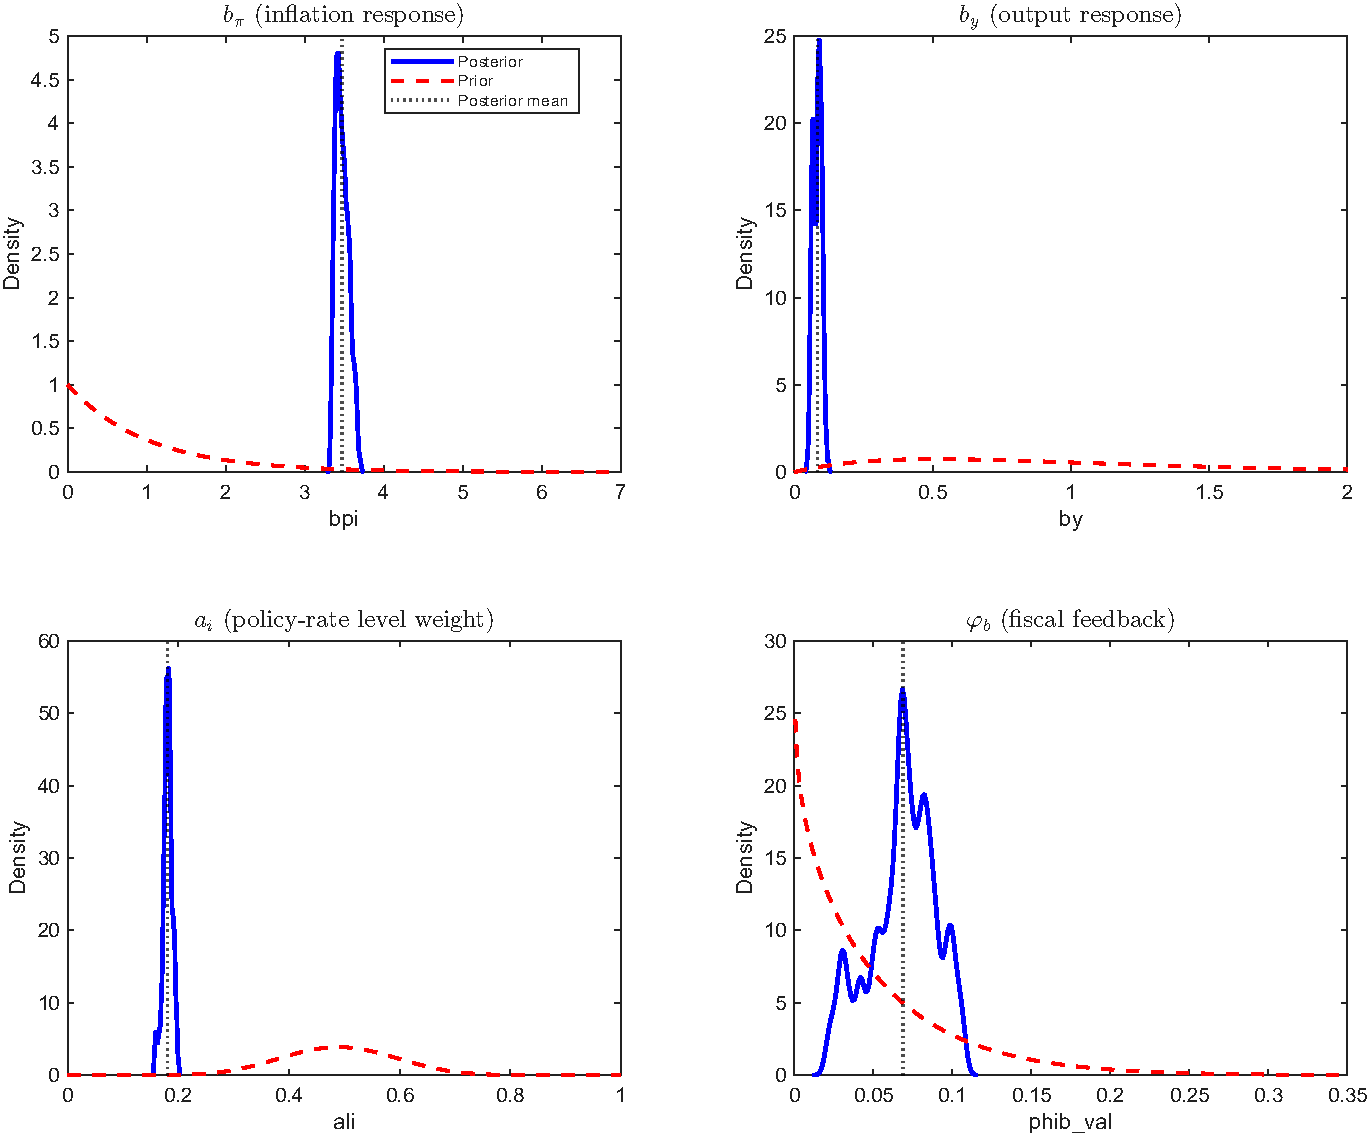
\includegraphics[width=0.85\textwidth]{prior_posterior_covid_bT_baa.pdf}
\caption{Prior (dashed red) and posterior (solid blue) densities for the
policy parameters $b_\pi$, $b_y$, $a_i$, and $\varphi_b$, current
(diffuse-prior) round. Dotted vertical lines mark the posterior mean.}
\label{fig:priorpost}
\end{figure}

The posterior for $b_\pi$ is tight and comfortably above unity even
under a prior with mean 1 and support well past 3, confirming the
Taylor principle is satisfied on the strength of the data rather than
the prior. The COVID labor-supply shock's standard deviation $\sigma_L$
again has a 90\% HPD interval well away from zero ([0.062, 0.076]),
against a deliberately loose prior (InvGamma(0.15,0.075)) chosen so that
a single-quarter outlier would not be crowded out by measurement error
absorbing it instead.

For reference, Table~\ref{tab:posteriors_old} reproduces the previous
(tight-prior) round's posterior estimates, under the pre-fix reserve
equation and the original $b_\pi,b_y,\varphi_b$ priors described in
Section~2.3.

\begin{table}[h]
\centering
\small
\begin{tabular}{lrrrl}
\toprule
Parameter & Prior mean & Post.\ mean & 90\% HPD & Prior \\
\midrule
$v^a$        & 2.500 & 2.776 & [1.526, 3.830] & Gamma(2.50, 0.75) \\
$\eta$       & 1.530 & 0.988 & [0.666, 1.266] & Gamma(1.53, 0.40) \\
$b_\pi$      & 2.100 & 2.169 & [2.015, 2.315] & Normal(2.10, 0.15) \\
$b_y$        & 0.280 & 0.135 & [0.068, 0.188] & Gamma(0.28, 0.10) \\
$a_i$        & 0.490 & 0.180 & [0.161, 0.199] & Beta(0.49, 0.10) \\
$b_r$        & 0.360 & 0.232 & [0.151, 0.333] & Beta(0.36, 0.10) \\
$\rho_z$     & 0.450 & 0.562 & [0.410, 0.720] & Beta(0.45, 0.10) \\
$\varphi_b$  & 0.100 & 0.094 & [0.066, 0.124] & Beta(0.10, 0.05) \\
\bottomrule
\end{tabular}
\caption{Previous round's posterior estimates (structural parameters
only), reproduced for comparison: pre-fix reserve equation, tight
$b_\pi,b_y,\varphi_b$ priors, custom pooled-posterior jumping
covariance, \texttt{mh\_jscale=0.25}.}
\label{tab:posteriors_old}
\end{table}

\section{Geweke (1992) Convergence Diagnostics}
\label{sec:geweke}

Table~\ref{tab:geweke} reports Geweke's convergence $p$-values (15\%
taper, $\chi^2$ test for equality of early- vs.\ late-chain means) for
the eight estimated structural parameters, computed separately for each
chain, for the accepted current-round (\texttt{hessian},
\texttt{mh\_jscale=0.05}) run. A parameter is classified as converged if
$p>0.05$.

\begin{table}[h]
\centering
\small
\begin{tabular}{lccccc}
\toprule
Parameter & Chain 1 $p$ & Converged? & Chain 2 $p$ & Converged? \\
\midrule
$v^a$        & 0.350 & Yes & 0.558 & Yes \\
$\eta$       & 0.088 & Yes & 0.008 & No  \\
$b_\pi$      & 0.062 & Yes & 0.089 & Yes \\
$b_y$        & 0.281 & Yes & 0.070 & Yes \\
$a_i$        & 0.024 & No  & 0.563 & Yes \\
$b_r$        & 0.001 & No  & 0.001 & No  \\
$\rho_z$     & 0.564 & Yes & 0.000 & No  \\
$\varphi_b$  & 0.226 & Yes & 0.081 & Yes \\
\bottomrule
\end{tabular}
\caption{Geweke convergence test $p$-values, 15\% taper, by chain
(current diffuse-prior round, \texttt{hessian} covariance,
\texttt{mh\_jscale=0.05}, $\bar\tau=0.14$, $\chi=0.5$).}
\label{tab:geweke}
\end{table}

This is the best convergence result of any round in this estimation
exercise: chain 1 passes 6 of 8 structural parameters, chain 2 passes 5
of 8 -- versus 6/8 and 4/8 for the previous round's best
(\texttt{posterior-cov}) result, and markedly better than the same
current round's own first production attempt at \texttt{mh\_jscale=0.10}
(2/8 and 3/8; see Table~\ref{tab:jscale2}), which motivated the further
jscale cut. $b_\pi$ now passes on \emph{both} chains, despite its
posterior having moved substantially under the diffuse prior -- the
convergence result is not an artifact of the prior pinning the estimate
near a fixed value. $a_i$ and $\rho_z$ fail on one chain each (having
each passed on both chains in the previous round), and $b_r$ fails on
both chains, roughly matching the previous round's pattern for that
parameter. $\eta$'s chain 2 failure ($p=0.008$) is the one parameter
that converged in the previous round but does not fully here; its
posterior HPD [0.922, 1.326] remains a reasonably tight, economically
sensible range regardless. As in every previous round, no single
jumping-covariance or jscale choice achieves full 8/8 convergence on
both chains simultaneously -- $b_r$ and (on one chain) $a_i,\rho_z$
remain the persistent stragglers here, analogous to $b_y$'s role in the
previous round.

\section{Determinacy and Expectational Stability}
\label{sec:detestab}

Determinacy (Blanchard and Kahn, 1980) and E-stability (Evans and
Honkapohja, 2001, Proposition 10.3) are evaluated on the RELAX-regime
linear model -- i.e., the model with $r^n_t = r^{n,notional}_t$ imposed
unconditionally, with no \texttt{occbin\_constraints} block and no ZLB
floor -- using a companion file,
\texttt{mmt8bOccBin3\_covid\_bT\_baa\_bkonly.mod}, that strips the
\texttt{estimated\_params}/\texttt{estimation(...)} machinery but
otherwise retains every shock from the estimated model, including
$\varepsilon^L_t$. Purely contemporaneous iid shocks with no own law of
motion do not enter the endogenous-variable Jacobian and therefore
cannot affect the Blanchard-Kahn eigenvalue count or the E-stability
spectral radius; what isolates the non-ZLB equilibrium is dropping the
OccBin regime-switching equation, not which shocks are declared.

All other parameters are held at their posterior means from
Table~\ref{tab:posteriors} (current, diffuse-prior round). The reserve
equation fix (Section~1) leaves this analysis mechanically unaffected --
$n_t$ does not enter the RELAX-regime Jacobian's forward-looking block
-- and was verified separately to leave the Blanchard-Kahn eigenvalue
count (4 forward-looking variables) and steady state unchanged.
Figure~\ref{fig:detestab} sweeps $(b_\pi, b_y) \in [0,5]\times[0,3]$ on a
$60\times 60$ grid -- the $b_\pi$ range extended from the earlier
rounds' $[0,3]$ specifically so the current round's posterior mean,
which the diffuse prior moved to $b_\pi=3.474$, actually falls inside
the plotted region rather than off its edge. Of the 3{,}600 grid points,
2{,}857 are simultaneously determinate and E-stable. The determinate and
E-stable classifications were verified to coincide exactly, cell-for-cell,
with zero mismatches across all 3{,}600 grid points, as expected from
Proposition 10.3 for this class of model. Because the two conditions are
literally identical here, they are combined into a single two-region
figure rather than shown as separate determinacy and E-stability panels.
At the posterior mean $(b_\pi,b_y) = (3.474, 0.083)$ the model is
determinate and E-stable -- comfortably inside the determinate region,
since the grid's own determinacy threshold along the $b_y=0.083$ line is
$b_\pi\approx1.10$ and the posterior mean sits more than three times
that value.

\begin{figure}[h]
\centering
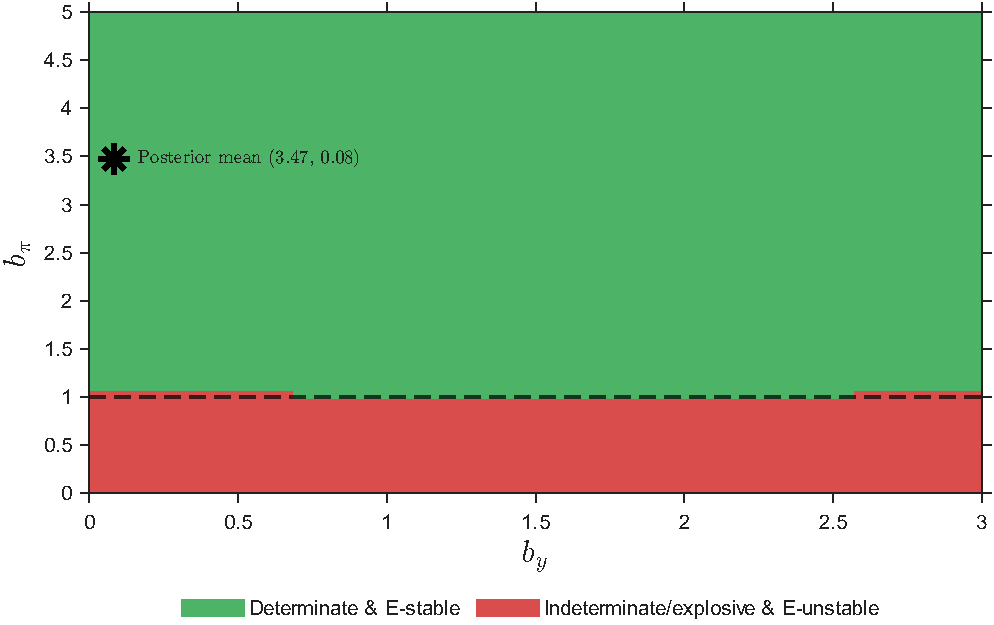
\includegraphics[width=0.65\textwidth]{det_estab_map_mmt8bOccBin3_covid_bT_baa.pdf}
\caption{Combined determinacy/E-stability region over
$(b_\pi,b_y)\in[0,5]\times[0,3]$, all other parameters at posterior
means (current, diffuse-prior round). Green: determinate \emph{and}
E-stable (the two conditions coincide exactly on this grid, with
0/3{,}600 mismatched cells). Red: indeterminate or explosive, and
E-unstable. The star marks the posterior mean
$(b_\pi,b_y)=(3.474,0.083)$, now visible within the plotted range.}
\label{fig:detestab}
\end{figure}

As a robustness check on the fiscal feedback parameter $\varphi_b$,
determinacy and E-stability were re-evaluated at
$\varphi_b \in \{0.0301,\ 0.0689,\ 0.1005\}$ (the current run's 90\% HPD
lower bound, posterior mean, and HPD upper bound), holding
$(b_\pi,b_y)$ at their posterior means:

\begin{center}
\begin{tabular}{@{}lccc@{}}
\toprule
$\varphi_b$ & Determinate? & Spectral radius & E-stable? \\
\midrule
0.0301 (HPD lower) & Yes & 0.9948 & Yes \\
0.0689 (posterior mean) & Yes & 0.9837 & Yes \\
0.1005 (HPD upper) & Yes & 0.9744 & Yes \\
\bottomrule
\end{tabular}
\end{center}

Stability holds at all three points, with the spectral radius falling
(i.e., stability strengthening) as $\varphi_b$ rises across this range,
as in every previous round. The spectral radii are somewhat closer to
the instability boundary (1.0) than in the previous round (which ranged
0.9674--0.9844 across its $\varphi_b$ HPD), consistent with this round's
lower $\varphi_b$ HPD range sitting closer to zero, but stability is not
in question at any of the three points.

\section{Steady-State Annualized Rates}

Table~\ref{tab:ss} reports the model's steady-state gross quarterly and
annualized rates evaluated at the full posterior mean parameter vector
(Table~\ref{tab:posteriors}, current diffuse-prior round), obtained by
re-solving the non-ZLB (RELAX) steady state with \texttt{resol()} after
loading the posterior means -- necessary because $v^a,\eta$ (which do
enter the steady state, unlike $b_\pi,b_y,a_i,b_r,\rho_z,\varphi_b$,
which affect only the model's log-linear dynamics around it) moved from
the previous round. As a consistency check, the steady-state real rate
satisfies the Euler equation exactly: $r^\ell/\pi = 1/\beta = 1.003311$.

\begin{table}[h]
\centering
\begin{tabular}{lccc}
\toprule
Symbol & Description & Gross quarterly & Annualized (\%) \\
\midrule
$\pi$   & Inflation                     & 1.008964 & 3.63  \\
$r^\ell$& Loan rate                     & 1.012304 & 5.01  \\
$r^d$   & Deposit rate                  & 1.004333 & 1.74  \\
$r^n$   & Policy rate (interest on reserves) & 1.002214 & 0.89  \\
\bottomrule
\end{tabular}
\caption{Steady-state gross quarterly rates and simple annualized
percentages ($(\text{rate}^4-1)\times 100$) at the posterior mean
parameter vector, non-ZLB (RELAX) regime, $\bar\tau=0.14$, $\chi=0.5$,
current (diffuse-prior) round.}
\label{tab:ss}
\end{table}

These are close to, but not identical to, the previous round's steady
state (3.79\% vs.\ 3.63\% inflation, 1.86\% vs.\ 1.74\% deposit rate) --
a modest shift consistent with $v^a$ and $\eta$'s posterior means moving
somewhat (Table~\ref{tab:posteriors} vs.\ Table~\ref{tab:posteriors_old})
while $\bar\tau,\chi,\beta$ and every other steady-state-relevant
calibrated parameter are unchanged; the reserve-equation fix itself
leaves the steady state exactly unchanged (verified directly -- see
Section~1). Both qualitative features noted in the previous round persist.
First, steady-state annual inflation (3.63\%) remains well above the
original ($\bar\tau=0.20$, $\chi=1.0$) calibration's 1.10\%, consistent
with the larger calibrated deficit ($\bar\tau$ lowered from 0.20 to
0.14) dominating the lower $\chi$'s inflation-reducing effect. Second,
the steady-state deposit rate $r^d$ remains positive (1.74\% annualized),
as in the previous round, in contrast to the fractionally negative
values seen under the original calibration. The discount factor
$\beta=0.9967$ was originally chosen so that the loan rate would clear a
2\% inflation target while keeping the deposit rate above the ZLB; under
the recalibrated $\bar\tau,\chi$ that margin remains comfortably
positive.

\end{document}
